\documentclass[ngerman,12pt,titlepage]{scrartcl}

\usepackage[ngerman]{babel}

\usepackage[T1]{fontenc}
\usepackage[utf8]{inputenc}
\usepackage{varioref}
\usepackage{hyperref}
\usepackage[ngerman]{cleveref}
\usepackage{makeidx}
\usepackage{csquotes}
\makeindex
\usepackage{graphicx}
\usepackage{listings}
\usepackage{color}
\usepackage{xcolor}
\usepackage[most]{tcolorbox}
\usepackage{amssymb}
\usepackage{lmodern}
\usepackage{caption,subcaption}
\usepackage{wrapfig}
\usepackage{pdfpages}

\title{Parkour im Sportunterricht}
\author{Luca Kiebel \and Luca Hartmann \and Julian Uphoff}
\date{\today}

% Im Dokument genutzte Makros
\newenvironment{hlbox}{\begin{tcolorbox}[enhanced,colback=white,colframe=white,sharpish corners,fuzzy halo=0.5mm with lightgray]}{\end{tcolorbox}}
\renewenvironment{bmatrix}
{ \begin{center} \begin{em} }
{ \end{em} \end{center} }

\usepackage[
  height=9in,      % height of the text block
  width=7in,       % width of the text block
  top=78pt,        % distance of the text block from the top of the page
  headheight=48pt, % height for the header block
  headsep=12pt,    % distance from the header block to the text block
  heightrounded,   % ensure an integer number of lines
]{geometry}
\usepackage{fancyhdr}
\pagestyle{fancy}
\fancyhf{} % clear all fields

\rhead{Luca Kiebel \\ Luca Hartmann \\ Julian Uphoff}
\chead{
\includegraphics[width=0.08\linewidth]{hbbk-logo}}
\lhead{Parkour im Sportunterricht}
\lfoot{ \leftmark}
\rfoot{Seite \thepage}

\begin{document}
\maketitle
\newpage

\section{Einleitung}
Bei Parkour geht es darum möglichst schnell und effizient von einem Punkt zum anderen zu gelangen.
Dabei kann man dies überall machen, ob in der Stat oder in der Natur.
Der Weg selbst ist egal, die Hindernisse dürfen nur nicht künstlich vereinfacht werden. Es geht schließlich darum mit dem vorhandenen Umfeld zurecht zu kommen.\\ Parcouring hingegen wir bei Veranstaltungen als eine Art Wettkampf ausgetragen. Es werden künstliche Hindernisse aufgestellt die möglichst schnell überwunden werden müssen. \\ Im Sportunterricht lässt sich Parcouring sehr gut einbringen. Es verbindet viele Elemente des Turnens mit Kondition und Körperkontrolle. Außerdem ist Parkour \enquote{cool}.

\section{Aufwärmen}
Wichtig sind beim Parkour vor allem die Arme und Beine. Beim Aufwärmen ergiebt es also Sinn sich darauf zu konzentrieren, dass diese aufgewärmt und gedehnt werden.  \\ Im ersten Schritt laufen die Schüler Runden um die Halle, in der Zeit bauen wir die Übungsstationen auf. Gelaufen wird zunächst für 5 Minuten normal und dann weitere 5 Minuten Schattenlauf, wo einer aus unserer Gruppe Übungen zu den beiden Schwerpunkten Beine und Arme vormacht. Diese sind:
\begin{itemize}
	\item Knee High. Diese Übung dehnt die Beine und bereitet auf folgende Sprünge vor.
	\item Butt Kicks. Diese Übung dehnt ebenfalls die Beine.
	\item Seitliches Überkreuzlaufen. Hiermit wird die Kondition trainiert.
	\item Laufen mit rotierenden Armen. Dient dem Dehnen der Schultern.
\end{itemize}
Nach dem Warmlaufen haben wir bereits die Stationen aufgebaut und beginnnen mit dem gemeinsamen Dehnen im Kreis. Hier dehnen wir zunächst mit unseren Mitschülern unsere Arme und Beine, besonders aber auch die Schultern und der Rücken. \\ Nach dem Dehnen machen wir mit der Einweisung in die einzelnen Disziplinen, die unsere Mitschüler lernen sollen weiter.

\newpage

\section{Parkour}
\subsection{Einweisung}
Um Parkour schnell und besonders auch sicher zu meistern muss man bei den Grundlagen anfangen. \\ Für das Teamspiel, welches wir für den zweiten Teil der Doppelstunde geplant haben, müssen unsere Mitschüler folgende grundlegende Fähigkeiten erlangen:

\begin{enumerate}
	\item Präzisionssprünge
	\begin{itemize}
		\item Auf Reckstangen
		\item Auf Bänke
		\item Auf Barren
	\end{itemize}
	\item Sprünge
	\begin{itemize}
		\item Hockwende
		\item Lazy Vault
		\item Speed Vault
	\end{itemize}
\item Rollen
\begin{itemize}
\item Powerrolle
\item Kastensprung mit Powerrolle
\end{itemize}
\end{enumerate}
Die einzelnen Disziplinen werden in Form von Stationen beigebracht. Diese stellen wir mit Stationskarten vor. Die Schüler sollen sich selbst aussuchen, wann sie welche Stationen benutzen und sich selbst die Zeit zum erlenen der Fähigkeiten einteilen. Bei den Stationen leisten wir Hilfestellung und erläutern bei Unklarheiten. \\

\subsection{Aufbau}
Wenn sich die Schüler mit den Stationen \enquote{angefreundet} haben bauen wir mit allen den Parkour auf, den wir mit dem Teamspiel Brennball verbinden. \\ In der Grafik wird der Aufbau des Spielfeldes dargestellt. Um ein Rechteckiges Feld wird ein Parkour aufgebaut, den Team A durchläuft. In dem Feld versucht Team B einen Ball möglichst schnell in den Brenner (obere mitte des Feldes) zu werfen. \\ Ein Spieler aus Team A wirft den Spielball in das Feld. Die Spieler von Team B versuchen möglichst schnell an den Ball zu kommen und diesen in den Brenner zu werfen. Dabei dürfen die Spieler aus Team B nicht eine (hier gepunktet dargestellte) Linie übertreten. Dadurch hat Team A etwas mehr Zeit. \\ Wurde der Ball von Team A geworfen rennt der Werfer los und veruscht so schnell wie möglich zu einem der Basen (grüner Kreis mit X) zu kommen. An diesen muss er sich entscheiden, ob er noch weiter rennen will oder dort bleibt. \\ Auf einer Basis wird der Spieler nicht \enquote{verbrannt} wenn Team B den Ball in den Brenner bekommt. Wird der Ball vom nächsten Spieler aus Team A geworfen können alle Spieler, die auf Basen stehen weiterlaufen. \\  Ziel des Spiels für Team A ist es möglichst schnell mit möglichst vielen Spielern den Parkour zu durchlaufen, die Aufgabe von Team B ist es dies zu verhindern.  
  
\begin{center}
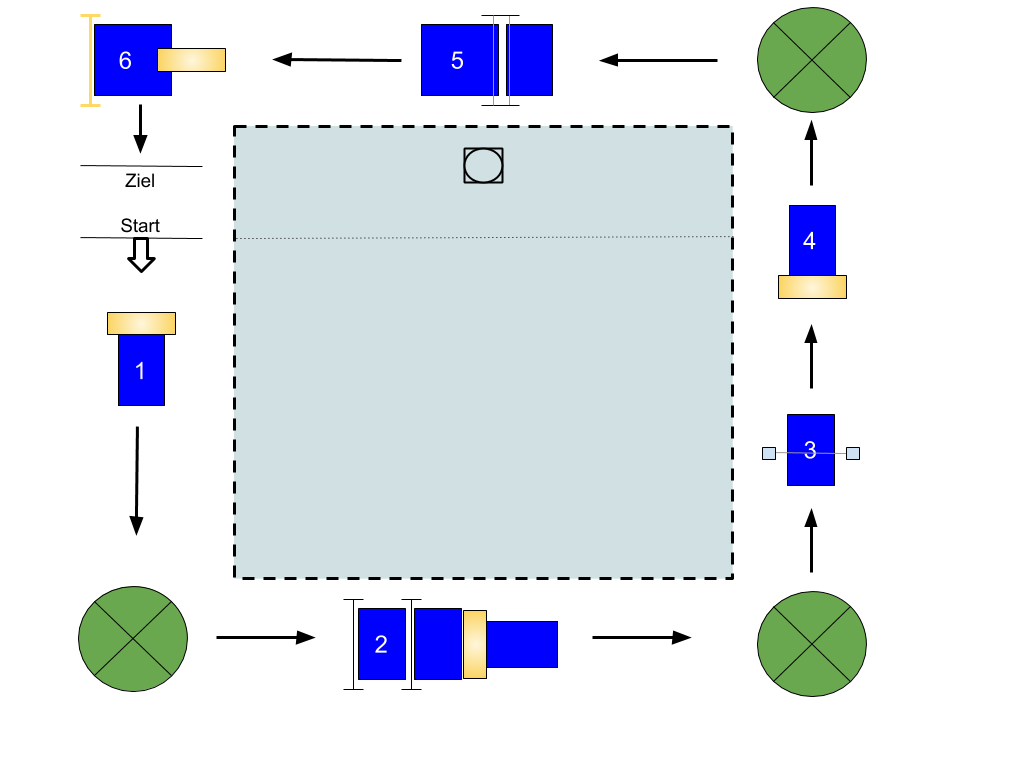
\includegraphics[width=0.9\linewidth]{brennball}
\end{center}
Das Spiel wird in zwei Runden gespielt, zwischen den Runden wechseln die Teams. Die Dauer der Runden legen wir vor Ort fest.
\\
Die einzelnen Stationen werden auf den folgenden Seiten (Stationskarten) genauer erklärt.

\newpage
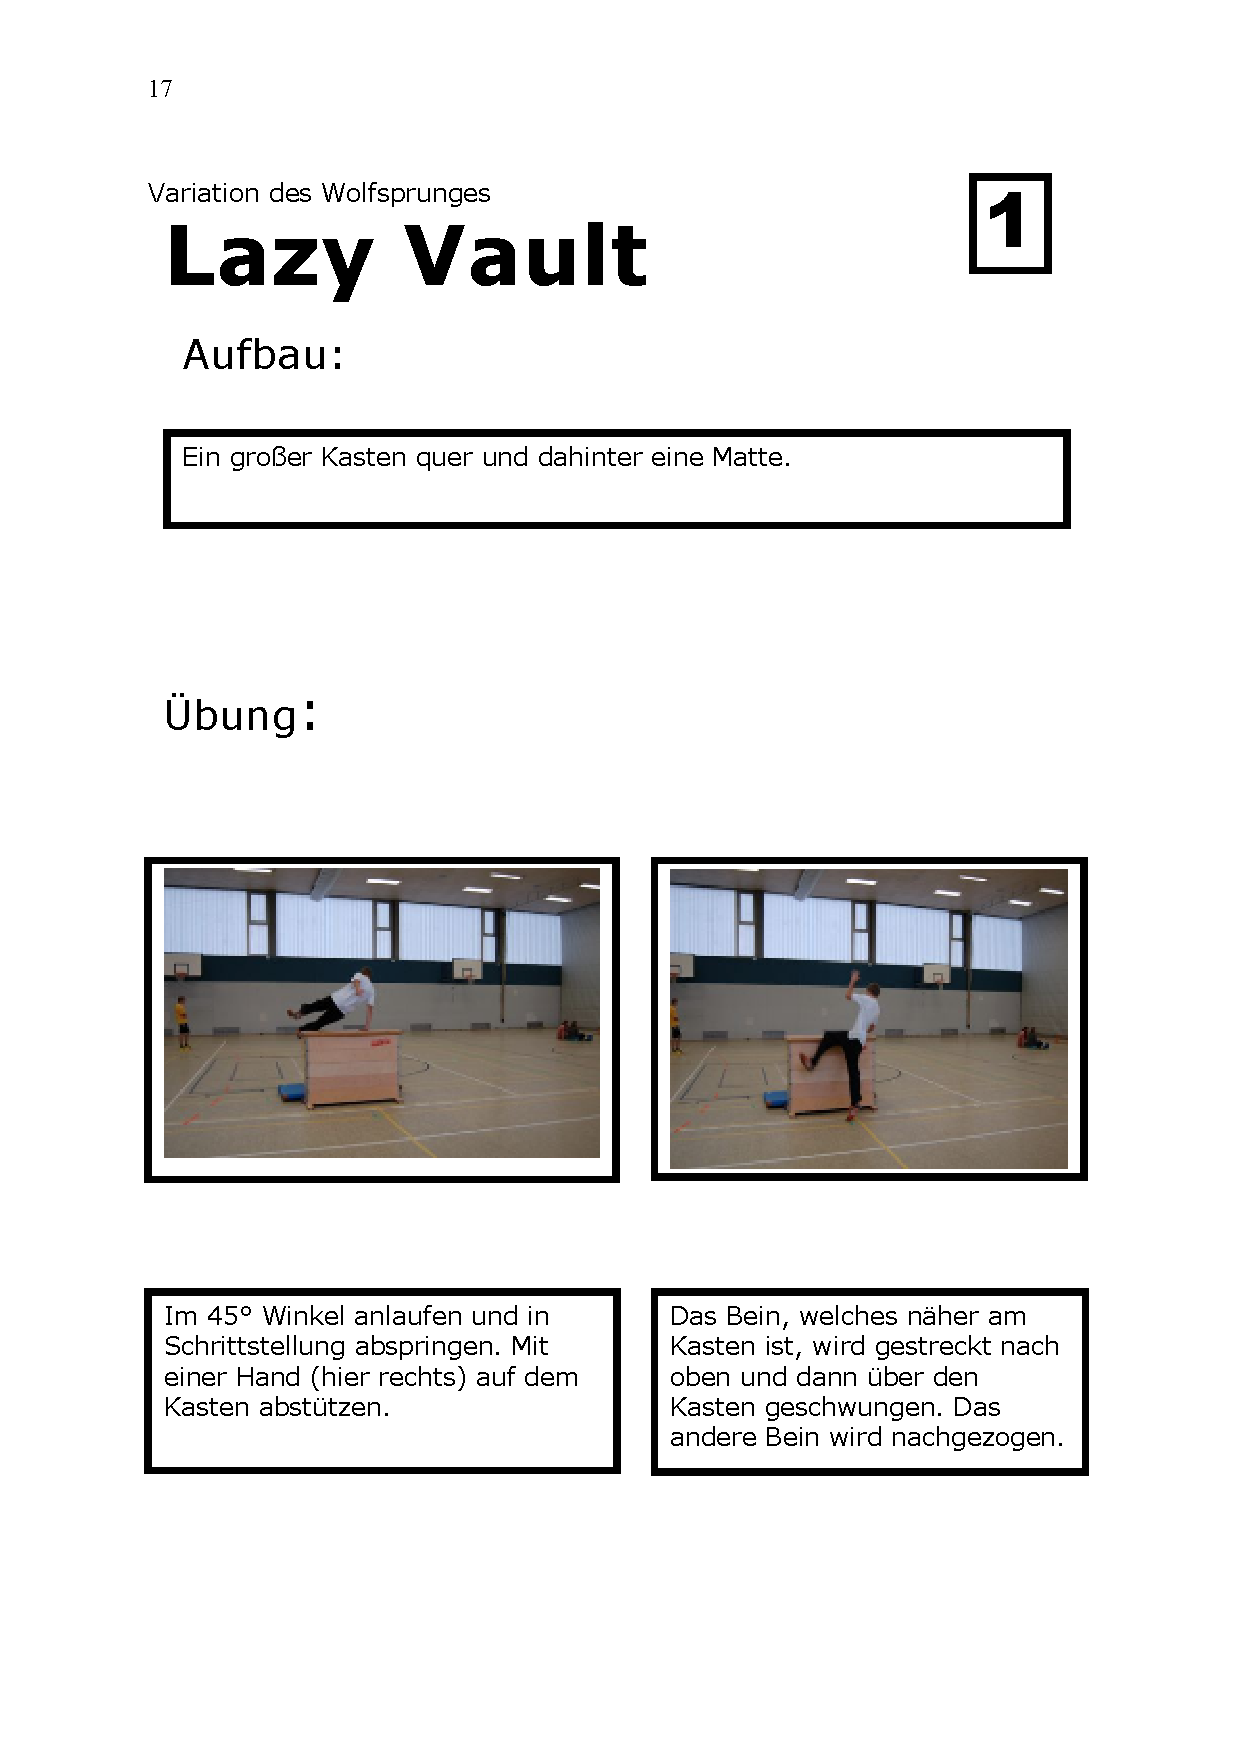
\includepdf[pages=-,pagecommand={},height=\textheight]{Stationen/01.pdf}
\newpage
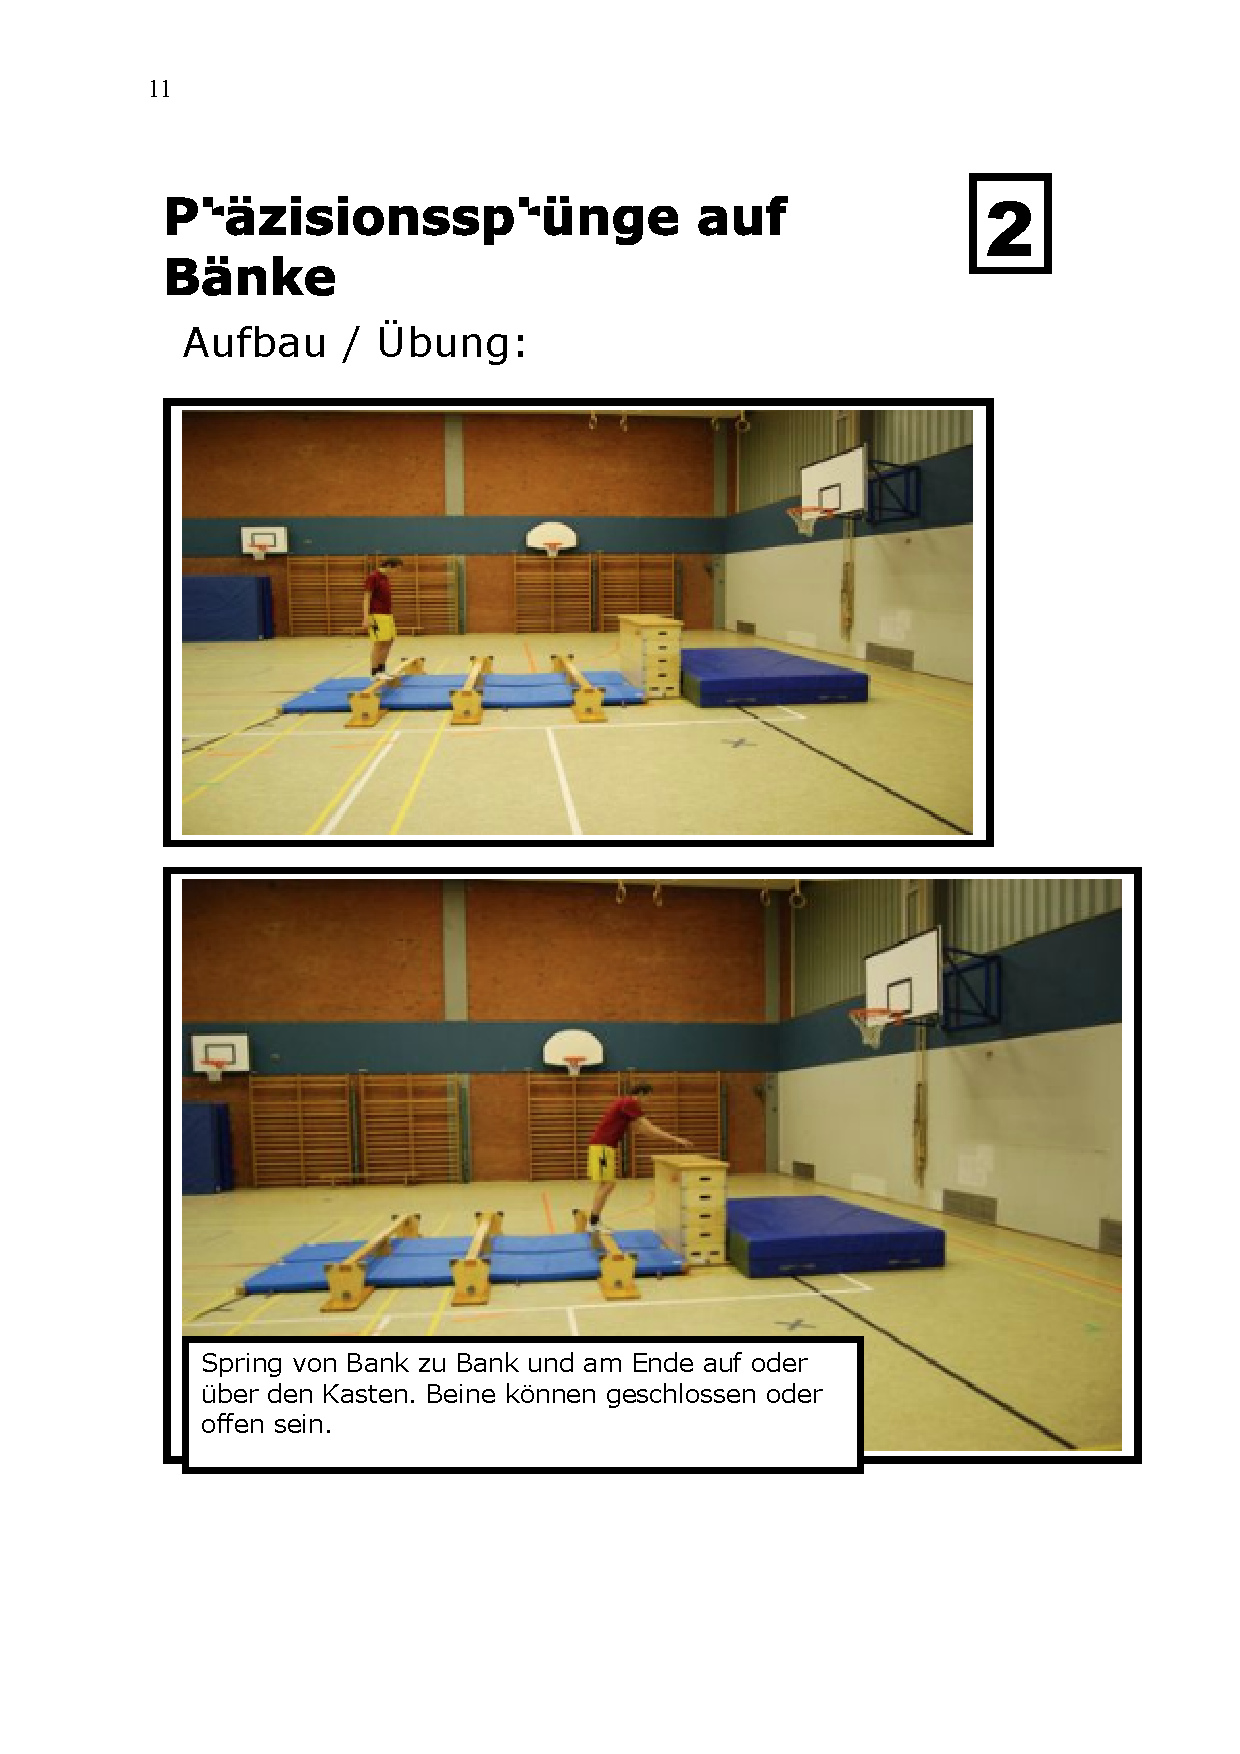
\includepdf[pages=-,pagecommand={},height=\textheight]{Stationen/02.pdf}
\newpage
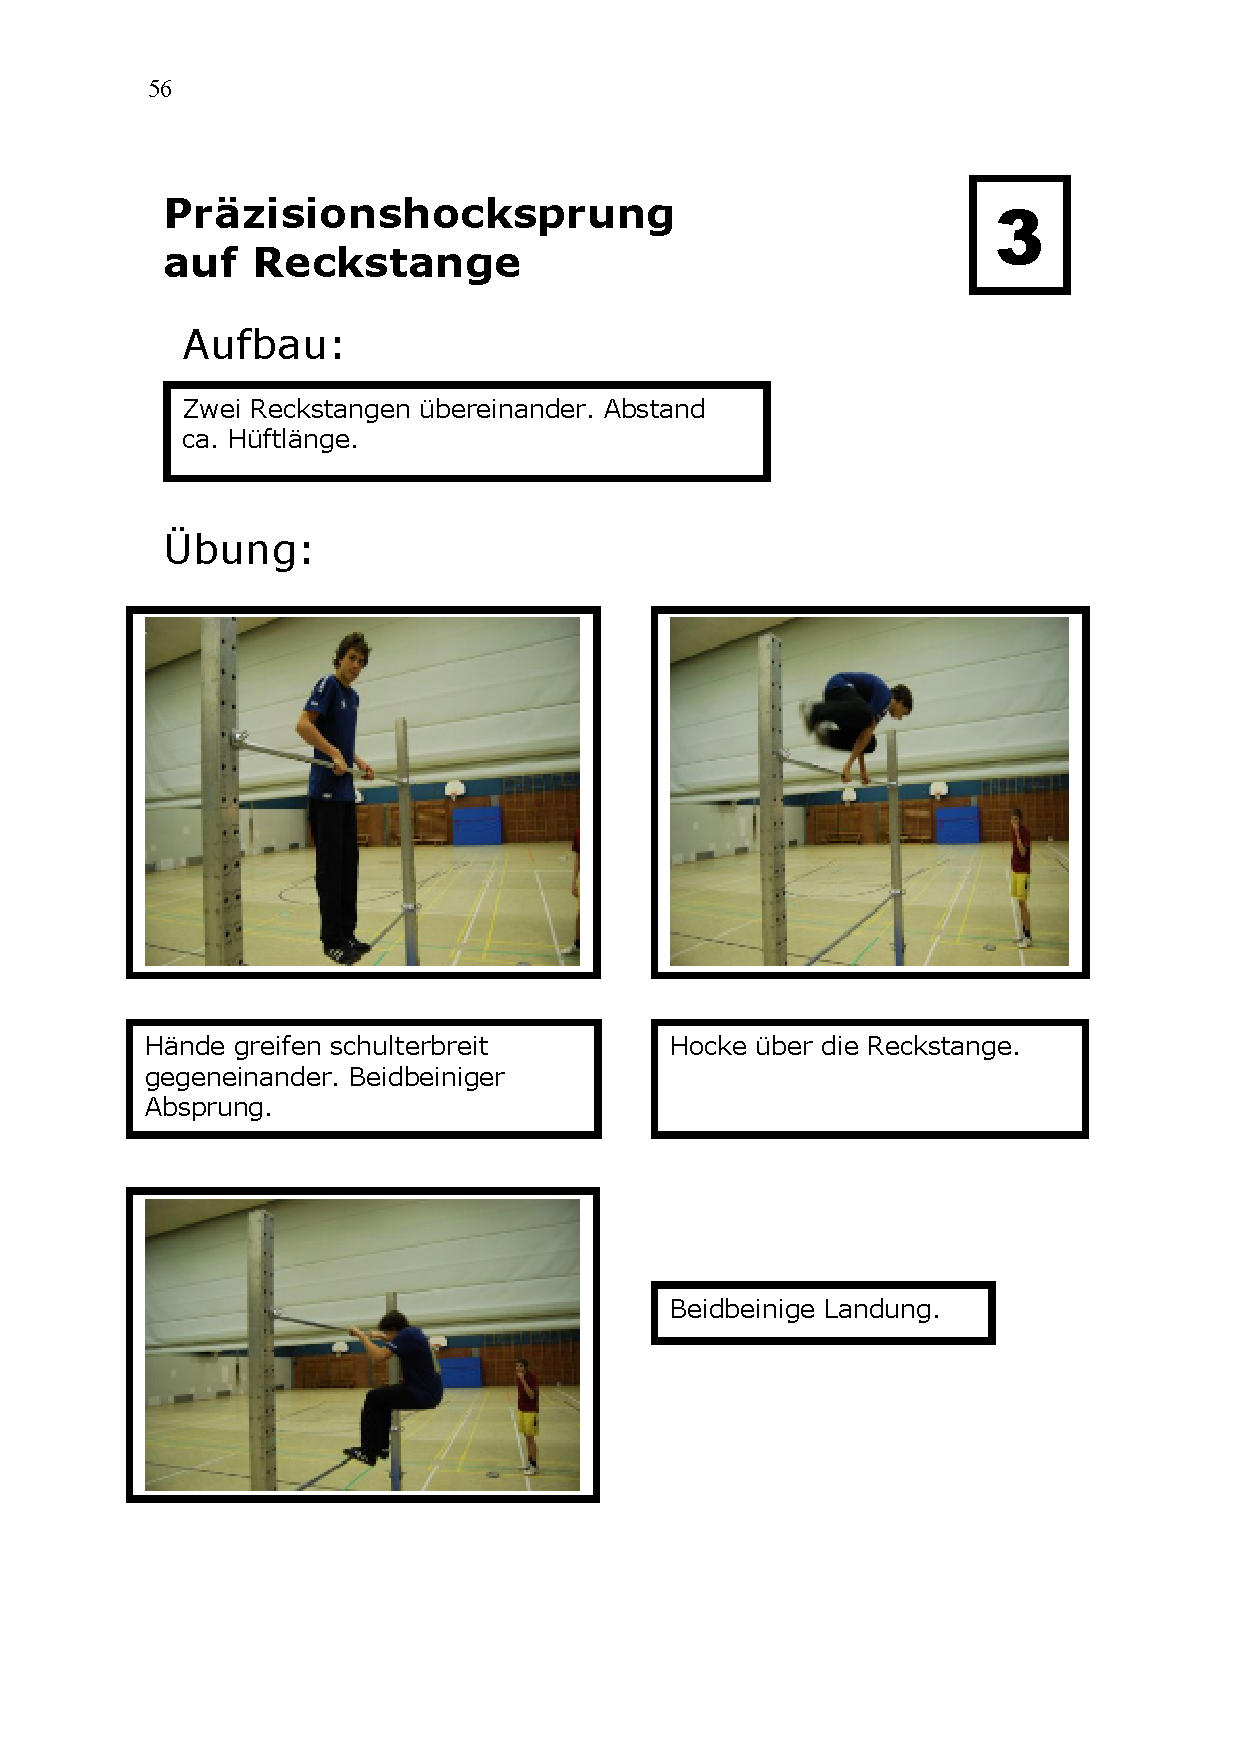
\includepdf[pages=-,pagecommand={},height=\textheight]{Stationen/03.pdf}
\newpage
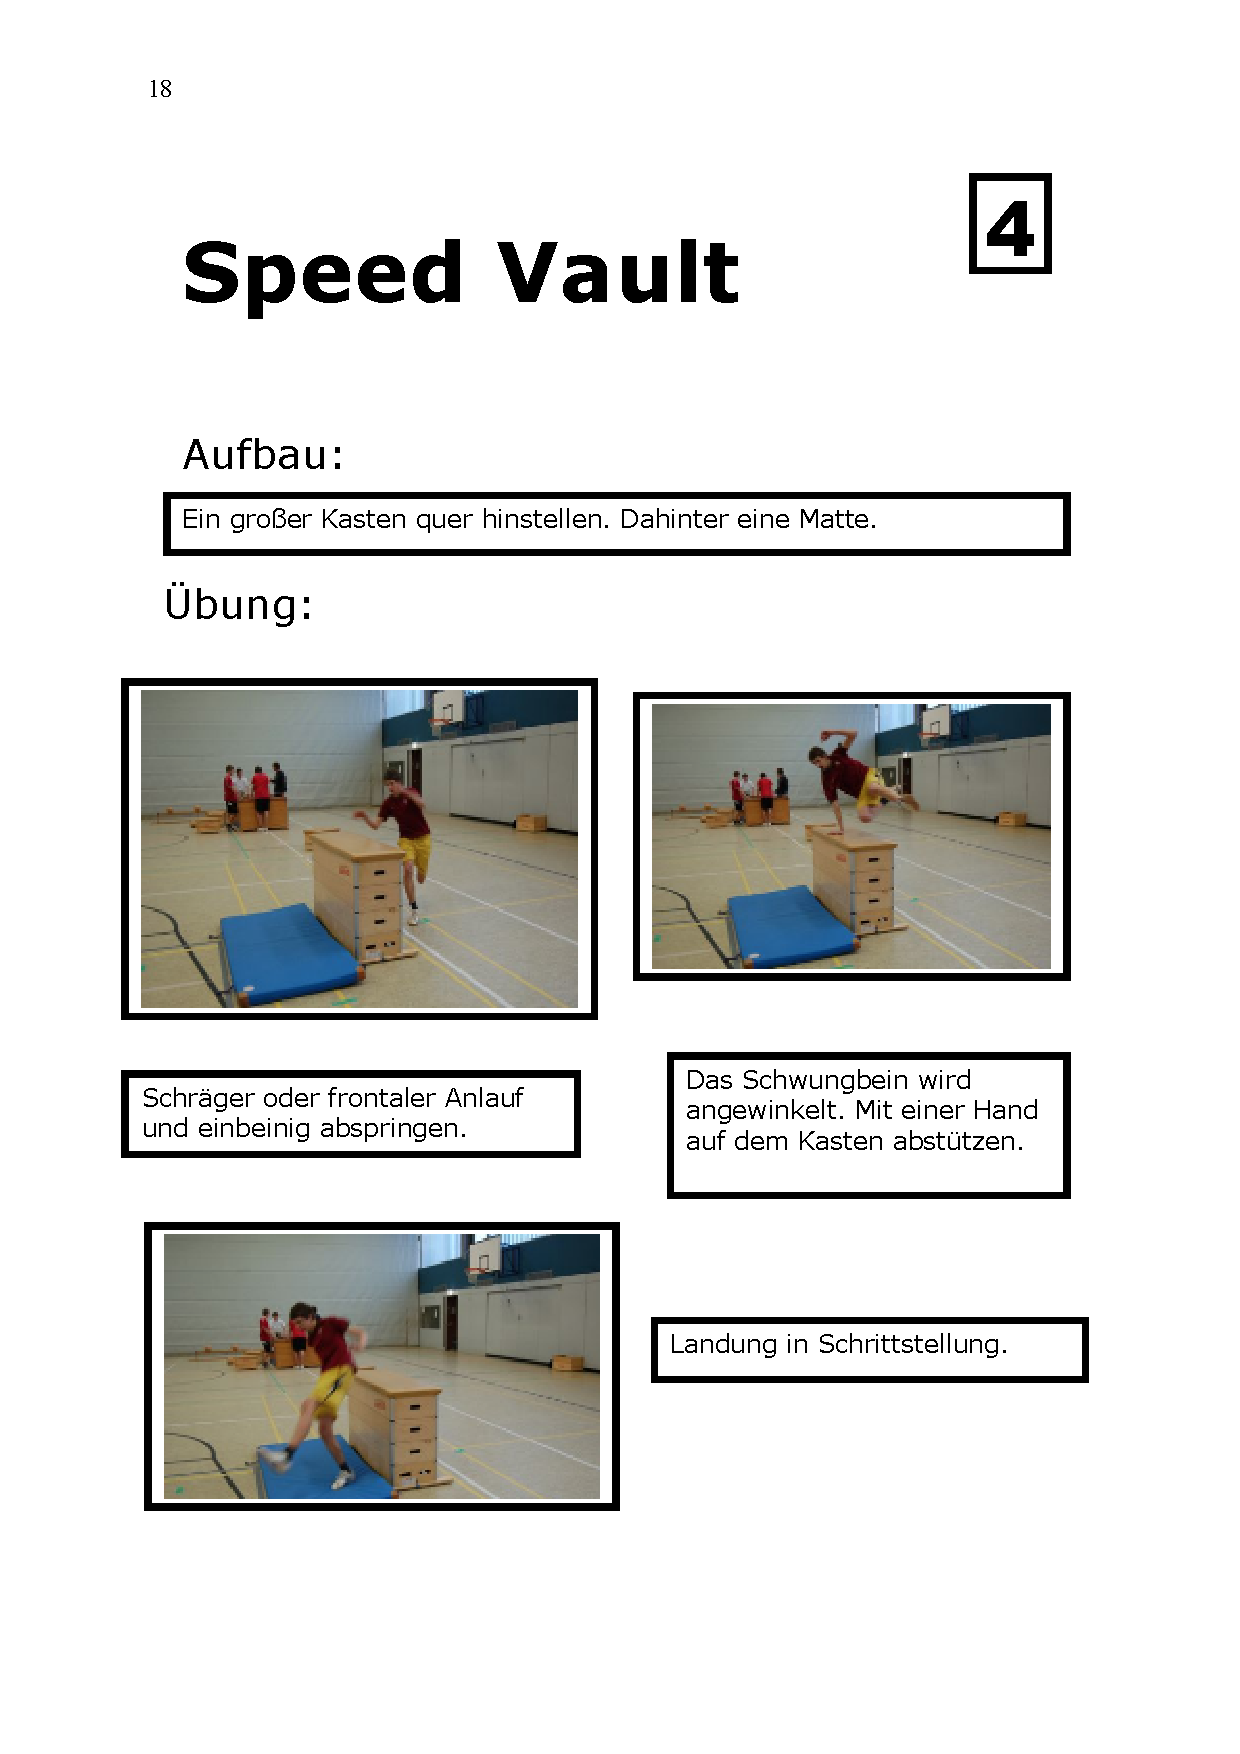
\includepdf[pages=-,pagecommand={},height=\textheight]{Stationen/04.pdf}
\newpage
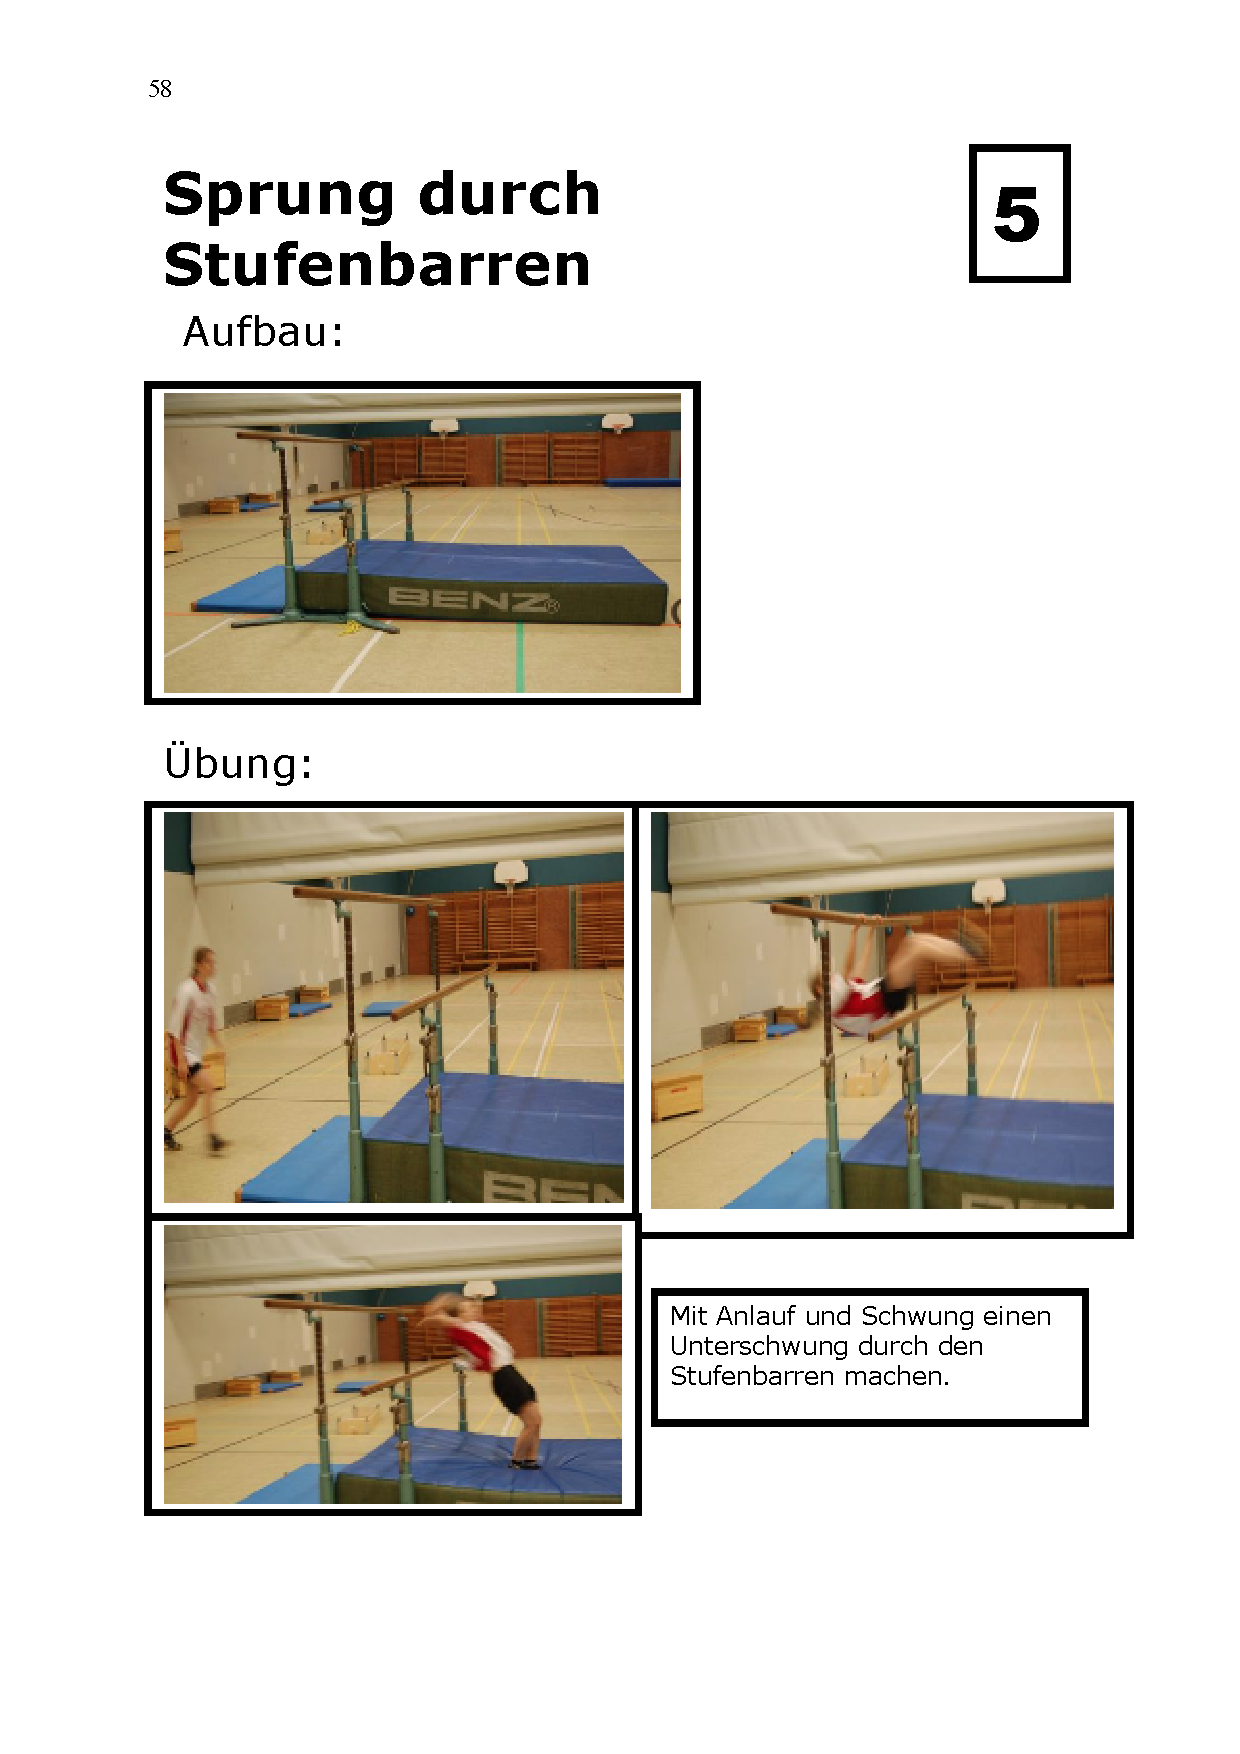
\includepdf[pages=-,pagecommand={},height=\textheight]{Stationen/05.pdf}
\newpage
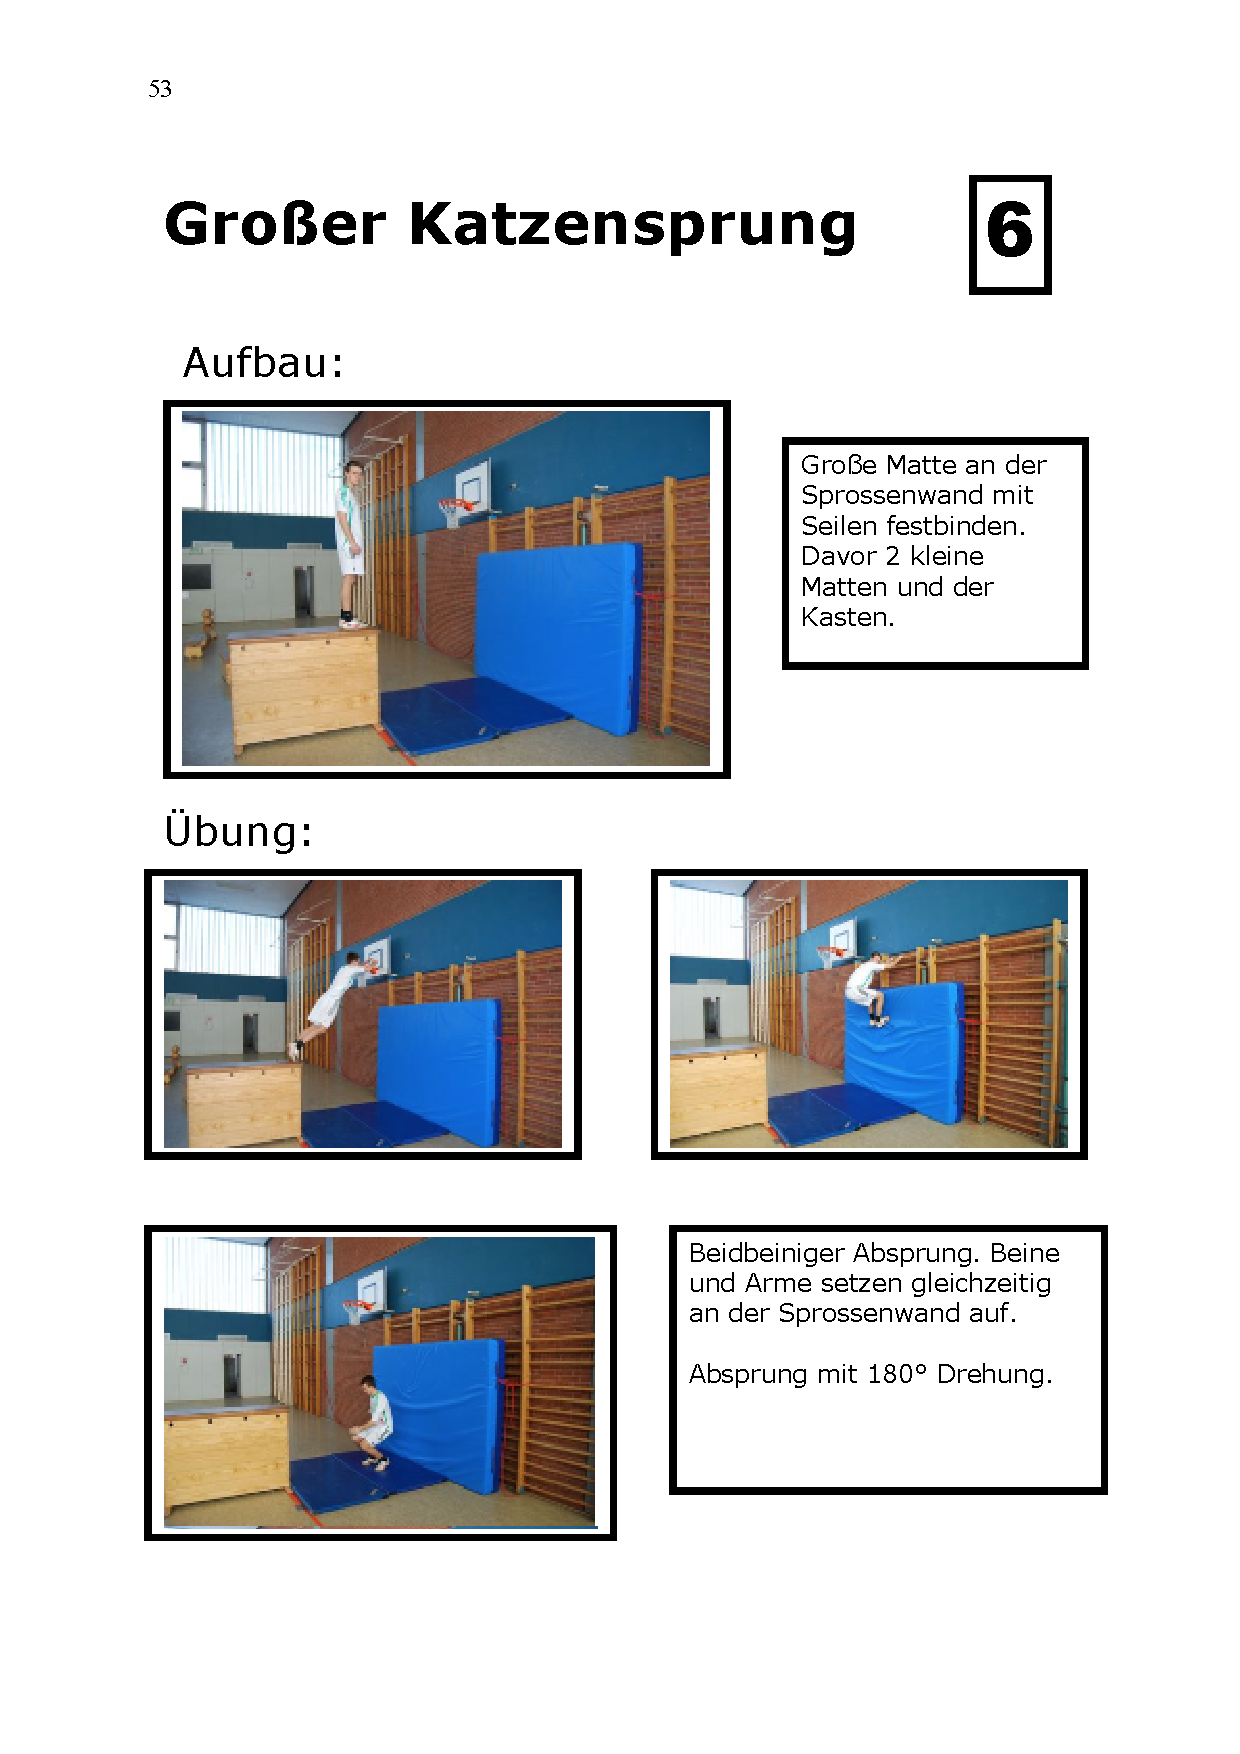
\includepdf[pages=-,pagecommand={},height=\textheight]{Stationen/06.pdf}

\end{document}
